\chapter{Simulation of Atmospheric Conditions over First Year Sea Ice using the Polar Weather Research and Forecasting Model}
\vspace{1 cm}
\begin{spacing}{1} \begin{quote} 
\noindent \emph{Current Arctic sea ice coverage levels (both annual and late summer) are at their lowest since at least 1850 (high confidence), and for late summer for the past 1000 years (medium confidence). Since the late 1970s, Arctic sea ice area and thickness have decreased in both summer and winter, with sea ice becoming younger, thinner and more dynamic (very high confidence).}\end{quote}
\hspace{6 cm} - IPCC Sixth Assessment Report, August 2021  
\end{spacing}
\vspace{1 cm}
\noindent 
\vspace{1 cm}\\
\noindent $^1$\\
$^2$\\
$^3$\\


\section*{Abstract}

\begin{spacing}{1} \noindent 
\end{spacing}

\doublespacing
\section{Introduction}

The Arctic has experienced large changes and dramatic loss in sea ice throughout the twenty-first century \citep{hines:2015}, signifying a transition in the Arctic from primarily thick, multi-year ice to thin, first-year sea ice. Increases in thin, first-year sea ice and open water have resulted in modeling errors not only in the polar regions but elsewhere on Earth \citep{hines:2015, royer:1990, francis:2009}. \citet{rinke:2006} found that specifying detailed sea ice information in models is key to predicting accurate atmospheric conditions. 

Polar WRF is a version of the Weather Research and Forecasting model (WRF) with modified physics for the polar regions. These modifications include enhanced mechanisms to allow prescribed sea ice thickness (default in non-polar WRF is 3 $m$), as well as sea ice fraction and snow depth \citep{hines:2015}. These mechanisms are primarily implemented in the land surface model (Noah LSM), but also include the heat transfer and thermal diffusivity through the snow and ice, albedo, snow density adjustments, and skin temperature calculations \citep{tastula:2012, hines:2015}. This model is the successor to Polar MM5 with advanced physical parameterizations \citep{bromwich:2009}. It has been used extensively for weather forecasting in Antarctica \citep{powers:2012} and has been tested over ice and land in the Arctic \citep{tastula:2012, bromwich:2009}. In spite of Polar WRF being available for over 10 years, the model has only undergone limited testing with no testing over young thin  sea ice. This paper  uses the comprehensive suite of instruments deployed during the Norwegian Young Sea Ice field campaign in 2015 (N-ICE) to test and evaluate the performance of Polar WRF over young thin sea ice. 


\section{Observations and Model Setup}

In this modeling study, observations from the Norwegian Young Sea Ice field campaign (N-ICE) were used to validate the Polar Weather Research and Forecasting model. The model was run for a 6-month period (1 January 2015 to 1 July 2015) for each combination of the selected CM and PBL schemes; this time period overlapped with the entire N-ICE campaign. Three case study periods were selected for further analysis using idealized model runs using radiosonde soundings taken during N-ICE as input.

\subsection{Observations}
N-ICE was a 6-month long research cruise that measured atmospheric and surface conditions from 15 January through 20 June 2015 \citep{granskog:2015}. Most notable for the analysis presented here are the atmospheric radiation measurements, taken by Kipp and Zonen (CMP22 and CGR4) radiometers at 1 to 1.2 $m$ above the ground. \citet{granskog:2015} and \citet{walden:2017} include a complete analysis of the radiative fluxes during N-ICE and includes a description of how surface temperatures were calculated. \citet{walden:2017} showed that the radiative fluxes during N-ICE were primarily influenced by wind, advection, and cloud cover. More details about the N-ICE field expedition can be found in Chapter 2.



\subsection{Model Setup}
The Weather Research and Forecasting model (WRF) version 4.1.4 was run with polar optimizations created by researchers at The Ohio State University. These optimizations include improvements of heat transfer over ice and updating sea ice fraction \citep{hines:2015}. These improvements have been tested over Arctic land and have had analysis done using SHEBA data, but have not yet been tested over first-year sea ice. The unique and large storms seen during N-ICE, along with the persistent surface temperature inversions present during the winter, make this dataset particularly interesting to use for Polar WRF validation.

\begin{figure}[H]
    \centering
    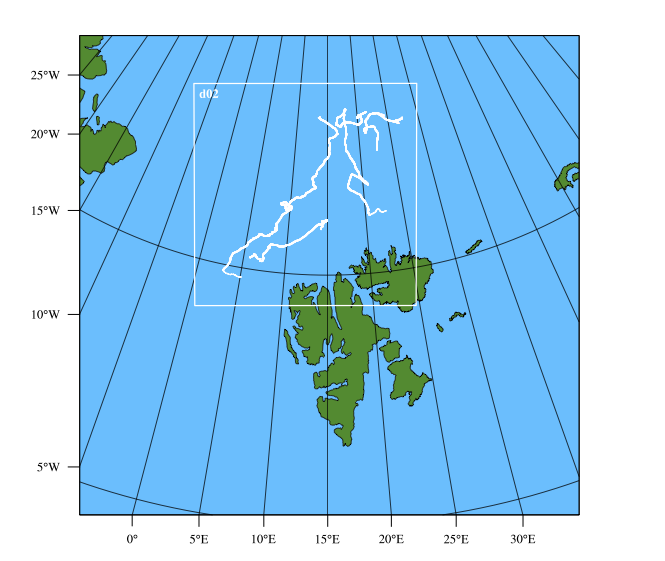
\includegraphics[width=1\linewidth]{figures/chapter3/wrf_domain.png}
    \caption[WRF Model Domain]{The WRF model domain with one nested domain (d02). The N-ICE ship tracks are in white.}
    \label{fig:wrf_domain}
\end{figure}

A 2-way nested two-domain setup was used and can be seen in Figure \ref{fig:wrf_domain}. The resolution domain of the nested domain is 3km by 3km, located just north of Svalbard and encompassing the entire spatial extent of the N-ICE field campaign. ERA-Interim was used for boundary and initial conditions, Pan-Arctic Ice Ocean Modeling and Assimilation System (PIOMAS) was used for snow depth, ice thickness, and albedo  \citep{PIOMASS}, and Special Sensor Microwave/Imager (SSMI) was input for ice extent information \cite{SSMI, schweiger:2011}. \citet{graham:2017} includes a comparison of the ERA-Interim dataset and the measurements taken during N-ICE. While \cite{graham:2017} found that ERA-Interim accurately portrayed the cloudy and clear states, there were still issues with the cloud liquid water path being underestimated, which should be taken into consideration when looking at the WRF results. The model was run for two periods, winter from January through March, and spring from April through June. Comparison with the N-ICE measurements for these periods start on 29 January and 24 April, resulting in 20+ days of spin-up time of the Polar WRF model before analysis. The simulations were completed using the Cheyenne supercomputer \citep{cheyenne}. More details about model settings are shown in Table \ref{tab:schemes}. 

\begin{table}[H]
\centering
\footnotesize
{
\begin{tabular}{| c | c |}
\hline
\rowcolor[HTML]{F3F3F3} \multicolumn{2}{|c|}{\textbf{Dates}} \\
\hline
Winter & 1 January - 1 April 2015 \\
Spring & 1 April - 1 July 2015 \\
\hline
 \rowcolor[HTML]{F3F3F3} \multicolumn{2}{|c|}{\textbf{Input Datasets}} \\
\hline
 Boundary and initial conditions & ETA-Interim \\
 Snow depth, ice thickness, and ice extent & PIOMASS and SSMI \\
\hline
\rowcolor[HTML]{F3F3F3} \multicolumn{2}{|c|}{\textbf{Polar WRF Settings}} \\
\hline
 LW and SW Radiation Scheme & RRTMG \\ 
 Surface Layer Scheme & Revised MM5 or ETA Similarity \\
 Land Surface & Unified Noah Land Surface Model \\ 
  \hline
\end{tabular}}
\caption{Input datasets and settings used for all Polar WRF simulations. ETA Similarity surface layer scheme was only used in cases with the MYJ BL scheme.}
\label{tab:setup}
\end{table}

In addition to the choice of input datasets and the underlying models used, one can select from a variety of different schemes to use with WRF. This study focuses on the evaluation of different planetary boundary layer (PBL) and cloud microphysics (CM) schemes because of their importance to Arctic conditions. The schemes used here were selected after a thorough literature review of previous WRF studies of both polar and non-polar applications. Various PBL schemes were selected to determine which of them most accurately represents the strong near-surface inversion in the Arctic. Clouds also have strong radiative importance in the Arctic, so a variety of CM schemes were selected to determine which provide accurate representations of Arctic clouds, including the presence of mixed-phase (water and ice) and supercooled water clouds. All other schemes, with the exception of the surface layer scheme, were kept constant throughout all simulations. Table \ref{tab:schemes} shows all PBL and CM schemes chosen for this study and the abbreviations used to refer to each model run. 

In addition to the PBL and CM schemes, a radiation scheme, surface layer scheme, and land surface model must be selected.  Unified Noah Land Surface Model (Noah LSM) was selected as the land surface model as this has been tested and improved over polar regions, and its tuning is a key strength of Polar WRF \citep{mukul:2004, hines:2015}. The Rapid Radiative Transer Model (RRTMG) was selected to handle longwave and shortwave radiation \cite{mlawer:1997} and the Revised MM5 surface layer scheme was used for all model simulations except those with the MYJ PBL scheme \citep{jimenez:2012}. The MYJ PBL scheme requires use with the ETA Similarity surface layer scheme as directed by the model \citep{janjic:2001}. 

\begin{table}[H]
\centering
\footnotesize
{\begin{tabular}{| c | c | c | c | c | c |}
  \hline
 \rowcolor[HTML]{F3F3F3} & & \multicolumn{4}{c|}{\textbf{CM Schemes}} \\
 \rowcolor[HTML]{F3F3F3} & & \textbf{Goddard} & \textbf{WRF 5-Class} & \textbf{Predicted Particle} & \textbf{Morrison 2-Moment} \\
  \hline
\cellcolor[HTML]{F3F3F3}
 &\textbf{YSU} & G-YSU & & P3-YSU & \\
\cellcolor[HTML]{F3F3F3}  & \textbf{MYJ} & G-MYJ & 5-MYJ & P3-MYJ & 2-MYJ \\ 
\cellcolor[HTML]{F3F3F3}  \parbox[t]{3mm}{\multirow{-3}{*}{\rotatebox[origin=c]{90}{\textbf{PBL}}}} \parbox[t]{2mm}{\multirow{-3}{*}{\rotatebox[origin=c]{90}{\textbf{Schemes}}}} & \textbf{MYNN} & G-MYNN & 5-MYNN & & 2-MYNN \\
  \hline
\end{tabular}}
\caption{Cloud microphysical (CM) and planetary boundary layer (PBL) schemes used for Polar WRF model simulations with corresponding abbreviations used to refer to each model run.}
\label{tab:schemes}
\end{table}

% Planetary boundary layer schemes
The most commonly used PBL schemes found in the literature were the Yonsei University (YSU) scheme \citep{hong:2004} and MYJ scheme. The Mellor–Yamada Nakanishi Niino (MYNN) scheme \citep{olson:2019} is a modified version of the Mellor–Yamada–Janjic (MYJ) scheme \citep{mesinger:1993}. The MYNN scheme has been tested over Svalbard, a location close to the N-ICE domain but with different surface conditions \citep{pilguj:2018}. Development of the MYNN scheme focused on large eddy diffusion \citep{cohen:2015}, while the MYJ scheme is focused more on stable flows \citep{janjic:1994, mellor:1982}. MYJ is a 1.5-order closure scheme and MYNN is a 2nd-order closure scheme \citep{pilguj:2018}.

% Cloud microphysical schemes
The Goddard (G) scheme \citep{tao:2000} and WRF Single-Moment 5-Class (5) scheme \citep{hong:2004} are the two most commonly used CM schemes found from the literature search regardless of the location being modeled. The Predicted Particle Properties (P3) scheme is a newly released scheme with advancements to the Morrison Bulk Two-Moment (2) scheme \citep{milbrandt:2016, morrison:2015}. This scheme was not designed for the polar regions, but is of particular interest due to the way it parameterizes ice particle density. Many CM schemes use bins to classify different cold cloud particle sizes and densities, leading to assumptions that can potentially lead to large errors. The P3 scheme eliminates the conversion between categories, reducing the simplifications for ice particles \citep{morrison:2005}. However, this scheme has a particle size cutoff, eliminating smaller particles, which may prove to be problematic in the dry polar regions.


\section{Results}

 Mean model bias (Eq. \ref{eq:modbias}) was calculated for skin temperature ($K$), latent heat flux ($Wm^{-2}$), sensible heat flux ($Wm^{-2}$), longwave radiation ($Wm^{-2}$), and shortwave radiation ($Wm^{-2}$) and is shown in Table \ref{tab:meanbias} for winter (top) and spring (bottom). Negative (positive) model biases indicate the model is producing values lower (higher) than those observed. The mean bias was selected as a way to determine model accuracy as it allows for a quick summary of how much the modeled time series disagrees with the measured values. The primary goal of this study is to determine which schemes perform well and which combinations of schemes give unreasonable values. A complete table with mean bias, correlation, and root mean square error is included in Table \ref{tab:wrfstats} in Appendix C.

\begin{equation}\label{eq:modbias}
Mean~bias = \frac{1}{n}\sum^{n}_{i=1}(y_{mod} - y_{obs})
\end{equation}


\begin{table*}[p]
\center
\centering
\vspace{-5em}
\footnotesize
\doublespacing
{
\begin{tabular}{| l | c | c | c | c | c |}
\hline
\rowcolor[HTML]{F3F3F3} & \multicolumn{5}{ c|}{\textbf{Winter}} \\
\rowcolor[HTML]{F3F3F3} & \textbf{Temperature} & \textbf{Latent Heat} & \textbf{Sensible Heat} & \textbf{Longwave} & \textbf{Shortwave} \\
\hline
\rowcolor[HTML]{F0F8E6}\textbf{G-YSU} & 0.3 & -1.0 & -23.4 & 2.9 &  \\
\rowcolor[HTML]{E0EDF4}\textbf{G-MYJ} & -0.1 & -0.3 & -22.6 & 4.4 & \\
\rowcolor[HTML]{FEEEF5}\textbf{G-MYNN} & 0.2 & -1.3 & -21.0 & 5.1 & \\
\rowcolor[HTML]{E0EDF4}\textbf{5-MYJ} & 0.7 & -0.8 & -23.0 & 3.4 & \\
\rowcolor[HTML]{FEEEF5}\textbf{5-MYNN} & 2.0 & -1.2 & -18.5 & 8.5 & \\
\rowcolor[HTML]{F0F8E6}\textbf{P3-YSU} & -7.5 & -1.1 & -25.0 & -2.5 & \\
\rowcolor[HTML]{E0EDF4}\textbf{P3-MYJ} & 3.1 & 0.4 & -17.2 & 12.9 & \\
\rowcolor[HTML]{E0EDF4}\textbf{2-MYJ} & 2.2 & -0.1 & -18.3 & 10.2 & \\
\rowcolor[HTML]{FEEEF5}\textbf{2-MYNN} & 4.5 & 0.1 & -17.1 & 12.0 & \\
\hline
\rowcolor[HTML]{F3F3F3} & \multicolumn{5}{c|}{\textbf{Spring}} \\
\rowcolor[HTML]{F3F3F3} & \textbf{Temperature} & \textbf{Latent Heat} & \textbf{Sensible Heat} & \textbf{Longwave} & \textbf{Shortwave} \\
\hline
\rowcolor[HTML]{F0F8E6}\textbf{G-YSU} & -2.6 & 2.3 & 2.2 & -33.0 & 2.2 \\
\rowcolor[HTML]{E0EDF4}\textbf{G-MYJ} & -2.4 & 2.0 & 2.0 & -32.0 & 2.0 \\
\rowcolor[HTML]{FEEEF5}\textbf{G-MYNN} & -1.8 & 2.7 & 4.1 & -27.1 & 4.1 \\
\rowcolor[HTML]{E0EDF4}\textbf{5-MYJ} & -2.0 & 2.7 & 4.0 & -29.2 & 4.0 \\
\rowcolor[HTML]{FEEEF5}\textbf{5-MYNN} & -0.7 & 3.3 & 6.3 & -22.0 & 6.3 \\
\rowcolor[HTML]{F0F8E6}\textbf{P3-YSU} & -9.4 & 3.3 & 6.1 & -32.2 & 6.1 \\
\rowcolor[HTML]{E0EDF4}\textbf{P3-MYJ} & -2.4 & 2.0 & 2.0 & -32.1 & 2.0 \\
\rowcolor[HTML]{E0EDF4}\textbf{2-MYJ} & -0.1 & 4.9 & 7.5 & -13.7 & 7.5 \\ 
\rowcolor[HTML]{FEEEF5}\textbf{2-MYNN} & 2.2 & 6.5 & 10.3 & -3.3 & 10.3\\
\hline
\end{tabular}
\caption{Mean model bias for temperature ($K$), latent heat flux ($Wm^{-2}$), sensible heat flux ($Wm^{-2}$), longwave radiation ($Wm^{-2}$), and shortwave radiation ($Wm^{-2}$). Acronyms in the left-hand column represent the MP and PBL schemes and are defined in table \ref{tab:schemes}. Rows are ordered by MP scheme and colored by PBL scheme for ease of use.}
\label{tab:meanbias}
\end{table*}}

\subsection{Skin Temperature}

Table \ref{tab:meanbias} shows the mean bias in model output compared to the N-ICE observations. G-MYNN and 2-MYJ had the smallest mean bias over the entire observation period. G-MYNN performed better in winter than in spring, and 2-MYJ performed better in spring. 2-MYJ had the lowest temperature bias in the spring, resulting in a smaller bias in longwave radiation. Figure \ref{fig:wrf_tsk} shows the distribution of skin temperature from each model run with the measurements shown in black. In the spring all model simulations produced cooler temperatures than were measured. P3-YSU produced the lowest skin temperatures throughout both the winter and spring, and as a result, had the largest bias temperature of all simulations.

Some of these disagreements between the model an measurements can be attributed to inaccurate surface albedo and a lack of cloudiness. The model simulated the surface albedo to be around 0.2 less than the measured surface albedo (0.6 compared to 0.8). The model surface temperature reaches the freezing point earlier than the model. The transition season is when the model had the most difficulty in simulating the skin temperature, but in the summer, when the temperature reaches freezing, all models and observations are in agreement.  There is a slight disagreement in the peak and magnitude of the peak around -30 $^{\circ}C$ between model runs. This shows that the model is not accurately representing clouds. It is assuming a warmer cloud radiative temperature indicating the clouds are warmer (lower) or that the cloud fraction is too high in the model. 

\begin{figure}[H]
    \centering
    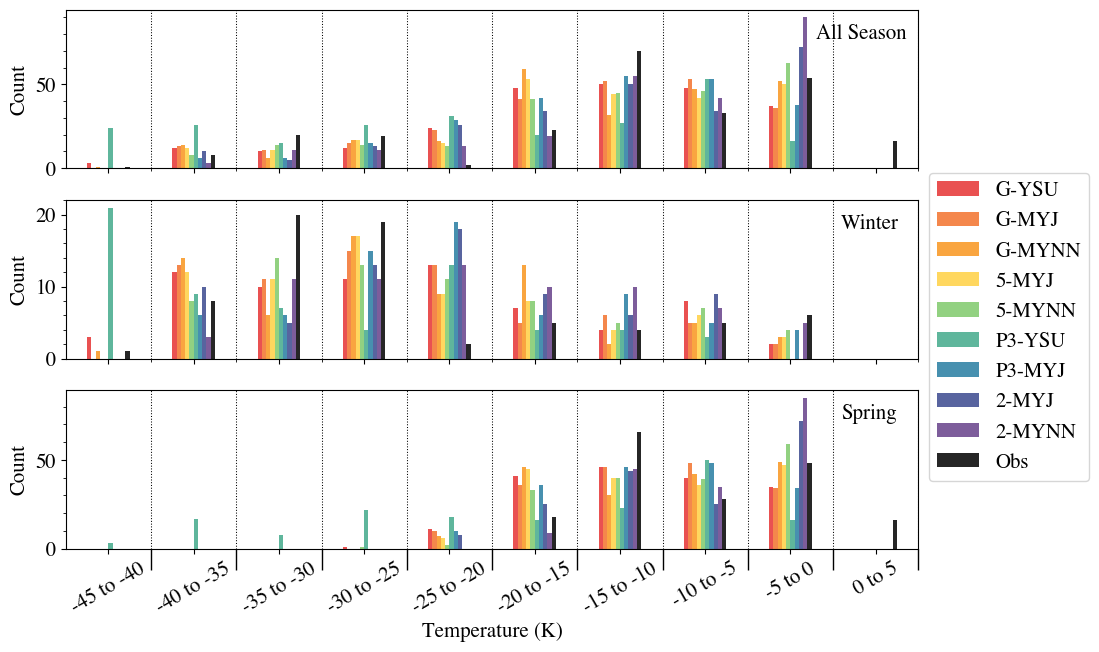
\includegraphics[width=1\linewidth]{figures/chapter3/WRF_TSK_Histo.png}
    \caption[Polar WRF simulation temperature histograms]{Temperature in winter (top), spring (middle), and for the entire observational period (bottom) for each of the Polar WRF runs. Measurements are shown in black.}
    \label{fig:wrf_tsk}
\end{figure}

\subsection{Longwave and Shortwave Fluxes}
 P3-YSU also had the largest bias in longwave radiation for the entire expedition (Figure \ref{fig:wrf_netlw}). However, for winter only, P3-YSU had the lowest bias in longwave radiation. All other model simulations produced a positive bias in the winter. This leads me to conclude this low bias in longwave radiation is likely the strong negative temperature bias compensating for the overestimation of longwave radiation occurring within the model. 

\begin{figure}[H]
    \centering
    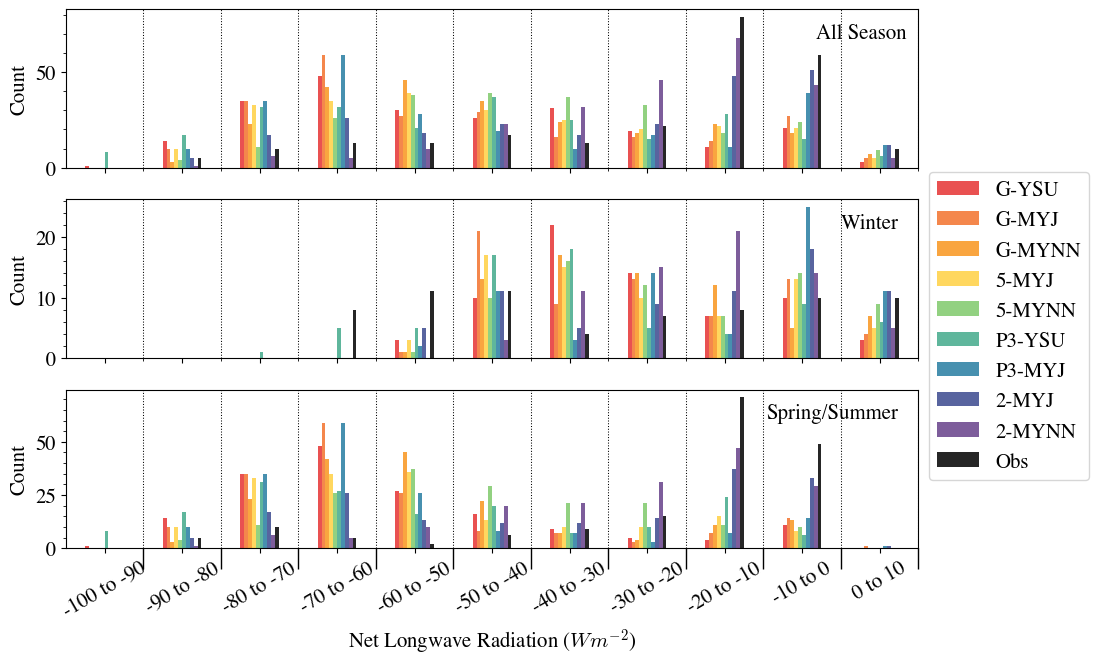
\includegraphics[width=1\linewidth]{figures/chapter3/WRF_NetLW_Histo.png}
    \caption[Polar WRF simulation net longwave radiation histograms]{Net longwave radiation in winter (top), spring (middle), and for the entire observational period (bottom) for each of the Polar WRF runs. Measurements are shown in black.}
    \label{fig:wrf_netlw}
\end{figure}
 
 The distributions shown in Figure \ref{fig:wrf_netlw} show two peaks. The first, a maximum around -60 $Wm^{-2}$ and the second around -10 $Wm^{-2}$. The first peak, the clear-sky peak, is most accurately captured by G-YSU. The second peak, however, is more accurately captured by 5-MYJ. 

In the spring, downward longwave is clearly dominated by the CM schemes as the schemes show different results, neither of which exactly match the measurements. Clouds in the spring were primarily thick, low-level clouds that radiate at relatively warm temperatures. This can be seen by the large peak in the measurements around 250 $Wm^{-2}$. The measurements, however, do not capture this large peak. There is one peak at higher radiation in all WRF runs but the magnitude not as large as that seen in the opaquely cloudy state for the measurements. The clear state has a similar peak amount of radiation but at a lower magnitude in the measurements compared to the model. This indicates that the model is not accurately portraying the portion of time that thick low-level clouds are over the area. Upward longwave radiation has a large peak around 250 $Wm^{-2}$ in the measurements with another secondary peak around 290 $Wm^{-2}$. The models do not capture these values well due to the incorrect resolution of the surface temperature. Net longwave radiation is incorrect due to the addition of errors in the upward and downward components. 

downward longwave radiation is portrayed well in most of the model runs except for the combination of the MYJ PBL scheme and the Goddard CM scheme in the Summer. However, even that scheme did capture the correct peak location. Upward longwave radiation, however, was slightly different in the model runs compared to the measurements. The measurements show a peak around 315 $Wm^{-2}$, while the model runs show this peak occurring at a slightly lower flux. All of the model runs captured this similarly, with less spread than the measurements.

\begin{figure}[H]
    \centering
    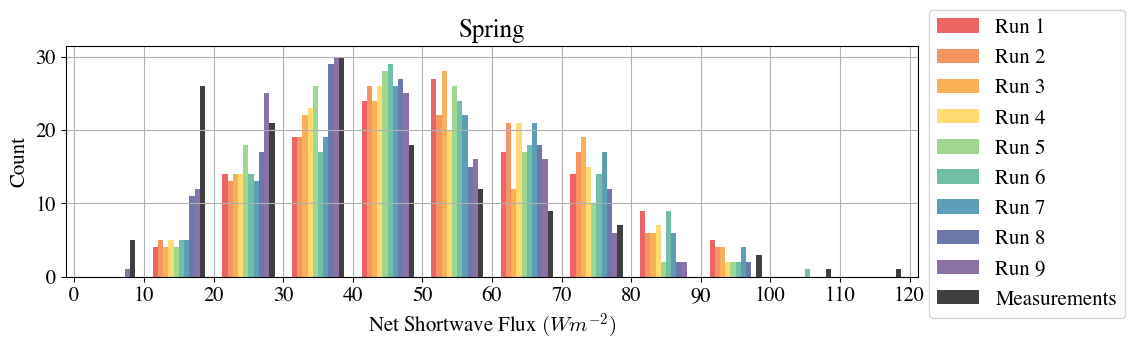
\includegraphics[width=1\linewidth]{figures/chapter3/WRF_NetSW_Histo.png}
    \caption[Polar WRF simulation net shortwave radiation histograms]{Net shortwave radiation in spring for each of the Polar WRF runs. Winter has been removed as shortwave radiation is zero.}
    \label{fig:wrf_netsw}
\end{figure}

Shortwave radiation (Figure \ref{fig:wrf_netsw}) is only shown and calculated for the spring period. The N-ICE location experienced 24-hour darkness in the winter until the sun rose in early March, at which time the hours of daylight increased until late April, at which time the sun stayed up 24 hours \citep{walden:2017}. The shortwave radiation is slightly larger in the model runs than in the measurements, with separation in the model runs by CM scheme. The distributions from the model runs peak at as much as 50 $Wm^{-2}$ higher than the measurements, with the peak of the distributions correlating with the CM scheme used. Because this time period had very limited clear-sky periods, it is likely that this peak had thin, high clouds occurring, and that the models are not resolving the cloud fraction correctly or are creating optically thinner clouds than are actually occurring. Additionally, the model has a low bias in upward shortwave radiation. The temperatures were warming during this period so this could be due to an incorrect albedo estimation. 

\begin{figure}[H]
    \centering
    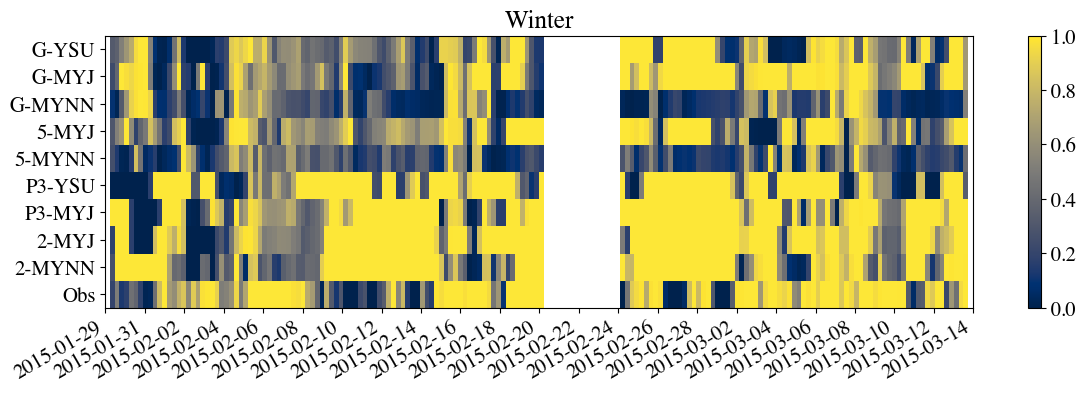
\includegraphics[width=1\linewidth]{figures/chapter3/WRF_CloudsWinter.png}
    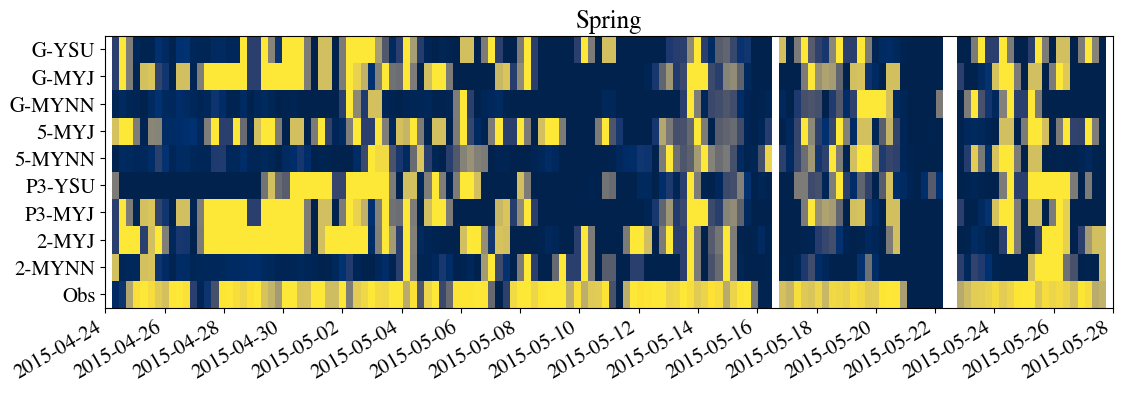
\includegraphics[width=1\linewidth]{figures/chapter3/WRF_CloudsSpring.png}
    \caption[Polar WRF simulation cloud fraction]{Cloud fraction from each Polar WRF run and the measurements in winter (top) and spring (bottom).}
\label{fig:wrf_cloudfrac}
\end{figure}

Cloud cover was consistently present, particularly in the summer. However, the radiation forcing in the model showed that either the cloud fraction was not high enough or the clouds were not optically thick enough in any of the simulations. Upward shortwave radiation was hindered by an unreasonably low surface albedo in the model simulations. This impacted the cloud radiative forcing as the upward shortwave radiation was less in the simulations than in the measurements. 


\begin{figure}[H]
    \centering
    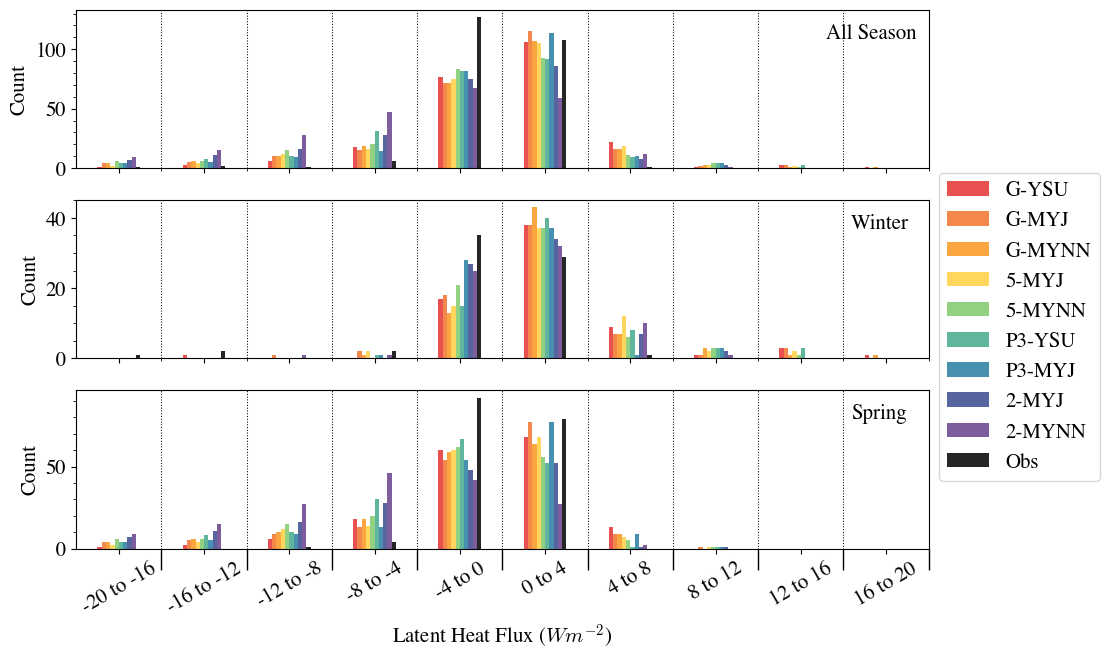
\includegraphics[width=1\linewidth]{figures/chapter3/WRF_LHF_Histo.png}
    \caption[Polar WRF simulation latent heat flux histograms]{Latent heat flux in winter (top), spring (middle), and for the entire observational period (bottom) for each of the Polar WRF runs. Measurements are shown in black.}
    \label{fig:wrf_hlf}
\end{figure}

\begin{figure}[H]
    \centering
    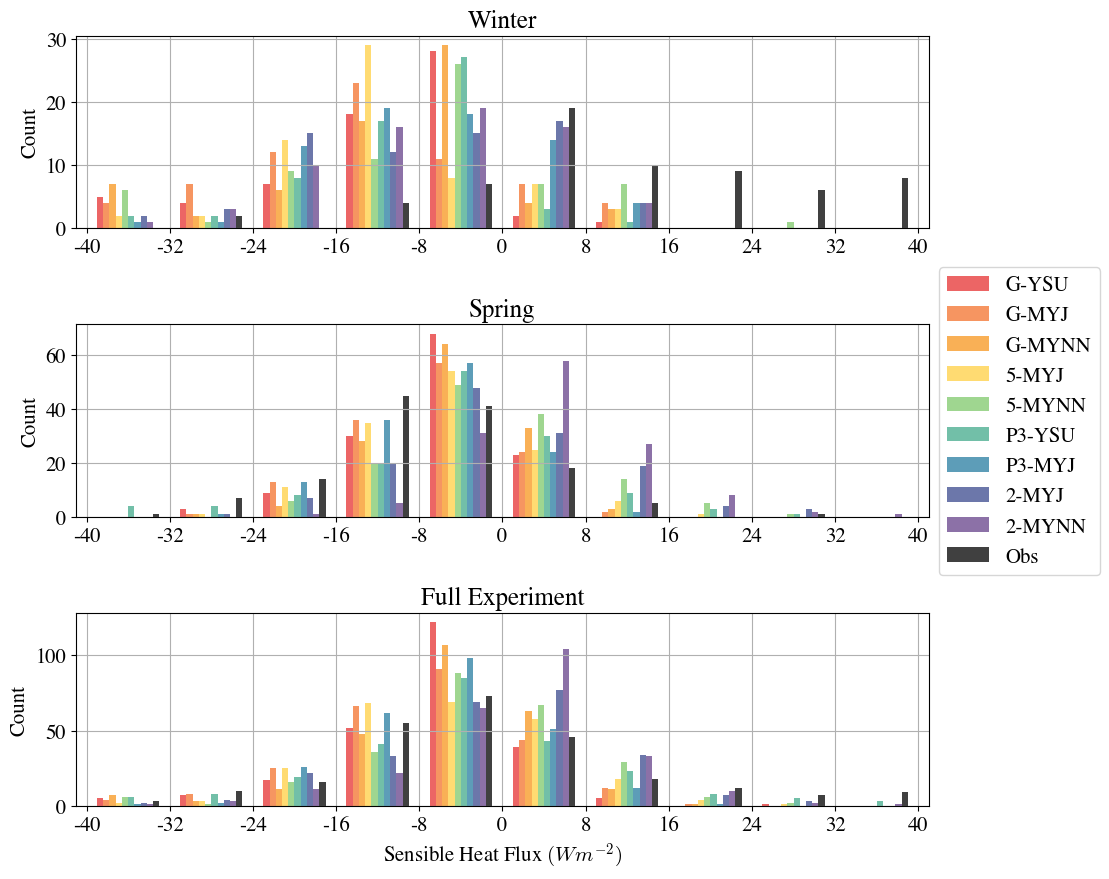
\includegraphics[width=1\linewidth]{figures/chapter3/WRF_SHF_Histo.png}
    \caption[Polar WRF simulation sensible heat flux histograms]{Sensible heat flux in winter (top), spring (middle), and for the entire observational period (bottom) for each of the Polar WRF runs. Measurements are shown in black.}
    \label{fig:wrf_shf}
\end{figure}

Figure \ref{fig:wrf_cloudfrac} shows the 6-hourly average cloud fraction in the grid cell corresponding to the ship location for each model run. The row labeled "Measurements" on each image is a 6-hourly vertical cloud fraction. This represents the percent of time in the 6-hour window that clouds were observed over the ship. While these are different metrics of calculating cloud fraction, they can still give a look into what the cloud cover was each day. For example, in the spring, cloud cover was seen almost the entire time; only one day can be classified as "clear sky." This day is 21 May, and can clearly be seen by the stripe of blue representing clear sky in the future. On the other hand, the winter saw less consistent cloud cover. Around 6 February, a period with cloud fractions closer to zero were observe in the measurements, but a range of cloud cover was produced by the model. P3-YSU, 2-MYJ, and 2-MYNN all produced complete cloud cover during this time, but other runs has cloud fractions closer to that seen at N-ICE. 

When comparing vertical cloud fraction to spatial grid cell cloud fraction the model simulations show less cloudiness than the measurements in the winter and more in the spring. The one period of extended clear sky in the winter (9 February to 15 February) was captured best by model runs using the Goddard or P3 CM schemes, with little apparent correlation to PBL scheme. The M3 storm period, which takes place from 15 February to 21 February, can be seen in the measurements as a period of 100 $\%$ cloud fraction almost the entire time. None of the simulations capture the high cloud fraction at the beginning of this storm period, but near the end of the storm period simulations using the P3 scheme and the Morrison Bulk 2-Moment scheme captured cloudiness. Later in the winter, however, the M4 storm (2 March to 4 March) is captured in its entirety quite well by both the P3 scheme and Morrison Bulk 2-Moment. However, near the end of the second Floe, all model runs show a decrease in cloudiness and a clear period, which was not seen in the measurements. 

The spring has an overall underestimation of cloud cover. There was only one day without cloud cover in the spring, 23 May, which was captured by all of the model runs. This is not surprising, though, as all runs show low cloud fraction throughout the entire season. This agrees with results seen by \citet{hines:2011} over Arctic land. This study showed that in the spring there were significant uncertainties and that simulations did not accurately represent the mostly cloudy conditions seen by the measurements. 

\subsection{Turbulent Fluxes}
Figures \ref{fig:wrf_hlf} and \ref{fig:wrf_shf} show the latent and sensible heat flux, respectively. The magnitude of latent heat flux was close to zero throughout the entire period, but modeled values reached up to -40 $Wm^{-2}$   at times in each of the different simulations. The spring and summer appeared to be the worst for the latent heat flux model calculations. 

5-MYJ, P3-YSU, 2-MYJ, and 2-MYNN did the worst at resolving the latent heat flux in the winter, as it showed a much larger spread with an accurate peak at 0 $Wm^{-2}$. This indicates more phase change than was actually observed. The YSU PBL scheme has a more narrow distribution during this time than the other PBL scheme, with an accurate (if not slightly more positive) peak. The peak shown by the YSU PBL scheme still has a wider distribution than the measurements with significantly higher positive values than the measurements, indicating this model is producing more deposition/freezing/condensation than is actually occurring.

Latent heat flux was similar in all the model simulations and was not close to the measurements in the spring. The measurements peaked at zero with limited spread, slightly favoring the negative values (melting/sublimation/evaporation). All the models, however, overestimated the amount of melting/sublimation/evaporation was occurring by overestimating the amount of negative latent heat flux. The models also have a much larger spread to them with a greater range of both positive and negative latent heat flux values, overall overestimating the phase change occurring.

Just as in other seasons, the summer latent heat flux is more largely negative with a larger spread in all the model simulations compared to the measurements. Measurements show values near zero with a small increase in the positive values (freezing/condensation/deposition) whereas the model runs favor a much larger amount of melting/sublimation/evaporation.

In the winter, sensible heat flux is incorrect in all model runs and is most influenced by the PBL scheme. The YSU PBL scheme shows a peak at the correct location, but a smaller spread than the measurements, indicating it does not create a surface temperature as different than the air temperature as the measurements are seeing. MYJ PBL, however, has the opposite problem. The spread is too large indicating the fluxes between the surface and atmosphere are too large, indicating larger temperature differences. Neither scheme accurately portrays the shape of the curve, which is less steep on the positive side.

Spring sensible heat flux peaked just below 0 $Wm^{-2}$ in the measurements, but were more negative in the model runs, indicating that the model predicted the atmosphere was warmer than the surface and flux was going into the surface. The MYJ PBL scheme predicted a small second peak slightly positive that was also captured in the measurements, but the shape, value, and magnitude of this peak was incorrectly portrayed in the model. This slightly positive peak occurred around 25 $Wm^{-2}$   in the measurements and was likely due to cold air advecting over the warming surface. The YSU PBL scheme did not capture this.

Sensible heat flux is captured well in the YSU PBL scheme simulations but not as well in the MYJ PBL scheme during the summer. The measurements and the YSU scheme runs showed a larger spread leaning slightly more into negative sensible heat fluxes, while the MYJ scheme had slightly more positive values and a more narrow distribution. This indicates that there is a greater flux into the surface in the YSU scheme and in the measurements, as the surface temperature is less than the air temperature.

\subsection{Case Studies}
\subsubsection{Case 1 - A Winter Cold Frontal Passage, 5 February 2015}

A cold front passed through the ship location just after midnight on 5 February, bringing a temperature drop of approximately 25 $^{\circ} C$. \citet{cohen:2017}, which defined major and minor storms during the N-ICE according to pressure and wind changes, indicated this was the second major storm that passed over the ship during the observation period. More information about the synoptic setup can be found in \citet{cohen:2017} and details about the surface energy budget can be found in \citet{walden:2017}. 

\begin{figure}[p]
    \centering
    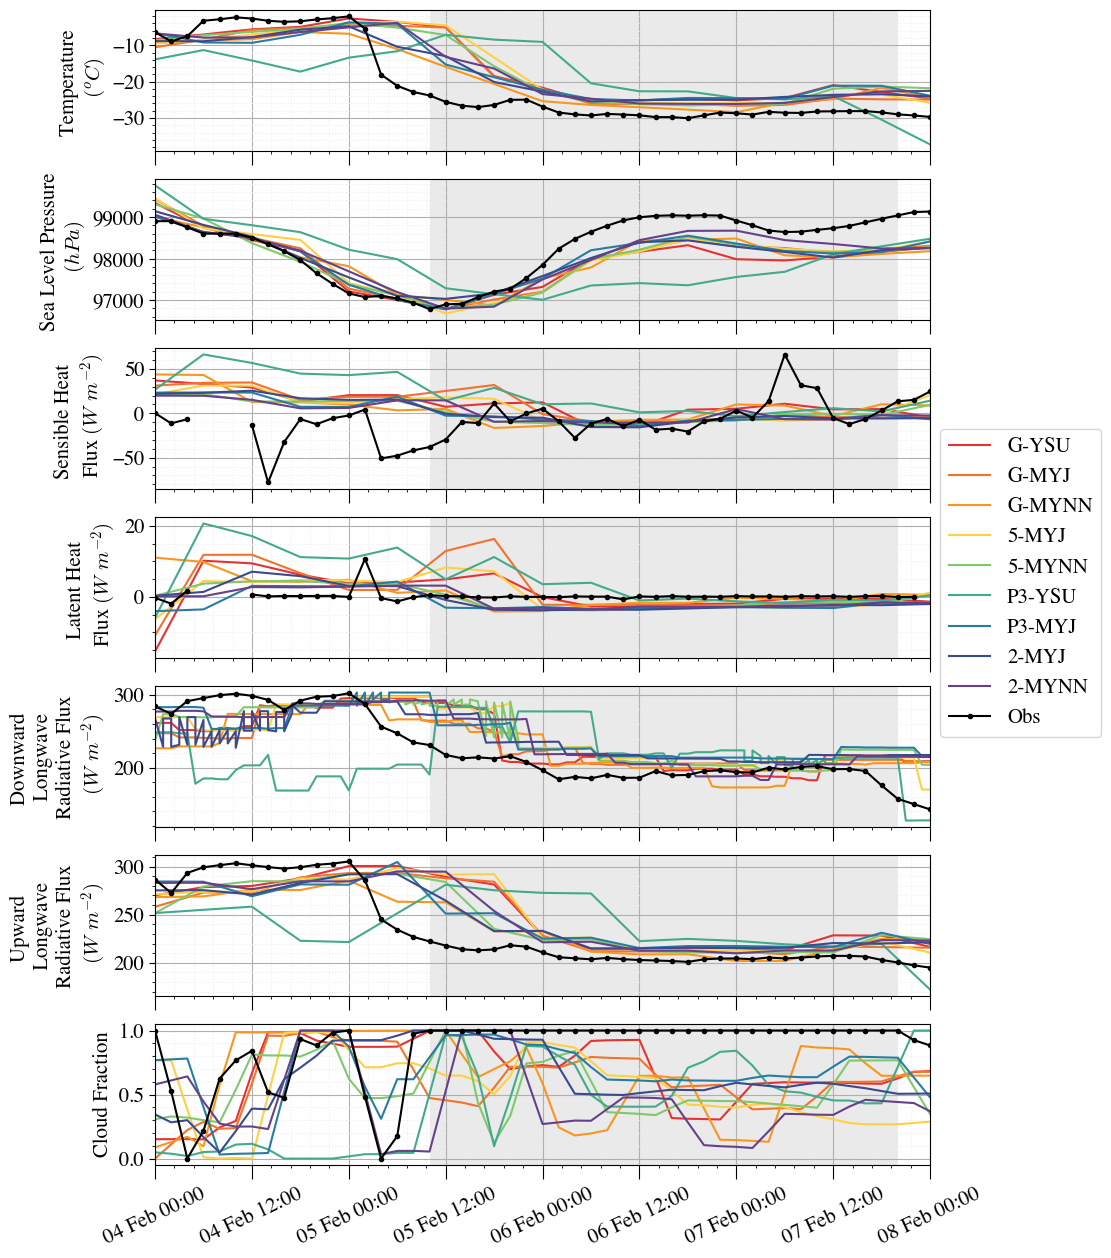
\includegraphics[width=1\linewidth]{figures/chapter3/wrf_case1.png}
    \caption[Polar WRF Case 1 - Winter cold front (5 Feb 2015) timeseries]{WRF model output (6-hourly, rainbow) and observations (2-hourly, black) for the period from 4 Feb to 8 Feb 2015 showing output variables during a cold front.}
    \label{fig:wrf_case1}
\end{figure}

The model output does not accurately capture the timing or magnitude of the cold front. Prior to the frontal passage, observed temperatures were warmer than those forecasted by WRF (top panel, Figure \ref{fig:wrf_case1}). Additionally, after the front passes, the modeled temperature is, at times, around 10 $^{\circ} C$ higher than the measured temperature. This can also be seen in both components of the longwave radiation (Figure \ref{fig:wrf_case1}, 5th and 6th panel from the top). P3-YSU performed particularly poorly during this period; this run had the lowest pre-frontal temperature and took the longest for temperatures to fall after the passage of the front.

A possible explanation for the P3-YSU scheme performing so poorly with temperature and longwave radiation is the lack of cloud cover before the front. This scheme consistently produced close to no cloud cover ahead of the front. While the observations did not see complete cloud cover until just after the front passes on 5 February at 12:00 (indicated by gray shading in Figure \ref{fig:wrf_case1}), the ship still experienced some cloud cover, at times approaching 100 $\%$ over the two-hourly averaging period. The P3-YSU scheme did not produce any cloud cover ahead of the front, and cloud cover reduced quickly after the frontal passage, which was not seen in the measurements. 

During the first half of this case, the sensible heat flux values in the measurements were negative, indicating that the surface was colder than the atmosphere. The model, however, produced positive sensible heat flux values during this time for all combinations of PBL and CM schemes. Latent heat flux is also largely positive in the models during this time, while the observations consistently observed latent heat flux values around zero. 

The schemes using the Morrison 2-Moment CM scheme performed the best in this case. These two consistently had cloud cover closest to the measurements during the first half of this case. They also performed the best for each of the other variables shown in Figure \ref{fig:wrf_case1} for the entire case, regardless of the reduction in cloud fraction each experienced during the second half of the case. How well the model simulates the fluxes, in this case, seems to depend on how well they can resolve the cloud fraction

\subsubsection{Case 2 - A Spring Clear-Sky Day, 23 May 2015}

Clouds were abundant during the spring at N-ICE. The only 25-hour clear-sky period occurred on 23 May. Observations and WRF output variables during this time can be seen in Figure \ref{fig:wrf_case2}. Unlike in the winter cold-front case, the Morrison 2-Moment schemes seem to be performing worse than the other schemes during this case. Temperatures in the simulations using the Morrison 2-Moment scheme were higher than the rest, with temperatures almost 20 $^{\circ} C$ above the observations being seen during the 10 hours of clouds seen on the 22nd prior to the start of the clear-sky period. Many of the schemes got the clear-sky period correct with the exception of the P3-YSU model run, which did produce some clouds mid-day on the 23rd. This run also had difficulties with the downward longwave throughout this period, with large jumps between values around 250 $W~m^{-2}$ and 190 $W~m^{-2}$. 

Model runs using the Goddard CM scheme perform best during the clear-sky period, with latent-heat flux values close to zero and longwave radiative flux values closest to the measurements. These schemes also had the most accurate temperature.

\begin{figure}[p]
    \centering
    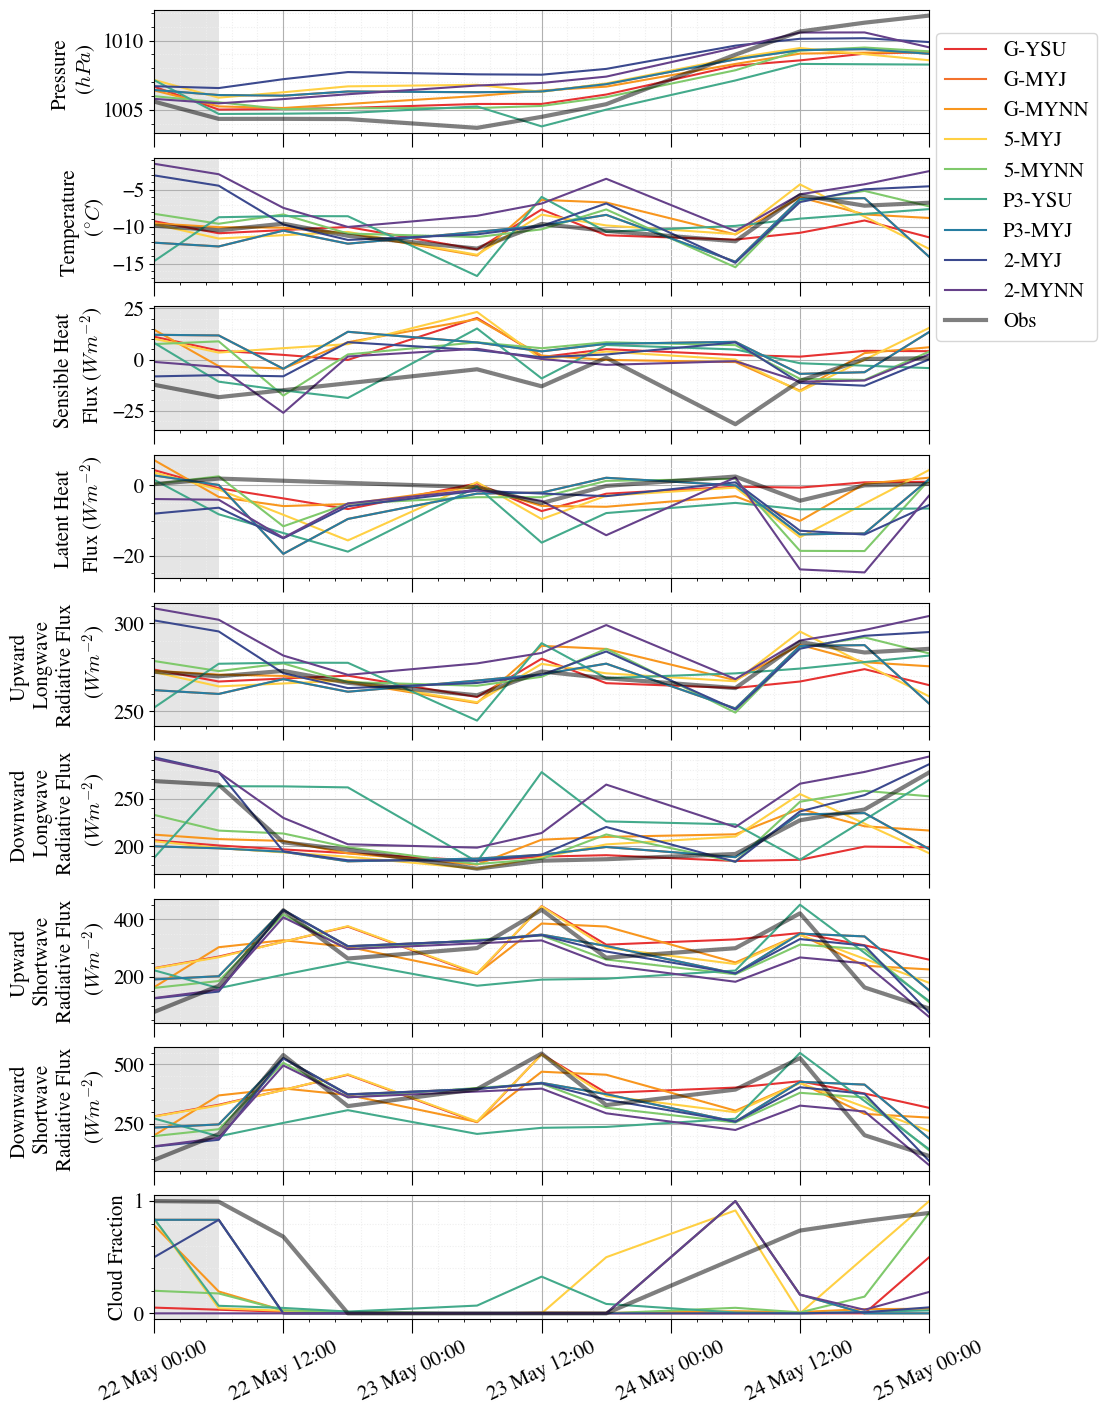
\includegraphics[width=1\linewidth]{figures/chapter3/wrf_case2.png}
    \caption[Polar WRF Case 3 - Spring clear-sky (23 May 2015) timeseries]{WRF model output (6-hourly, rainbow) and observations (2-hourly, black) for the period from 22 May to 25 May 2015 showing output variables during a spring clear-sky period.}
    \label{fig:wrf_case2}
\end{figure}

\section{Conclusions}

In this study, Polar WRF was used to simulate surface fluxes over first-year sea ice from January to June 2015. Model results were compared to observations taken during the N-ICE field campaign. CM and PBL schemes were selected based on the popularity of use in other modeling studies, but in the Arctic and elsewhere. 

The schemes using the Morrison 2-Moment CM had the lowest biases in latent heat flux in the winter overall and performed best in the winter cold front case study. However, the overall temperature biases from these schemes were the largest in the winter, indicating that these schemes perform best under conditions like those seen in the first case study. The P3 CM scheme performed the worst in the winter, with the highest biases in both longwave radiation, sensible heat flux, and temperature. This could be due to the cold temperature producing small cloud droplets that the scheme has not been tested or validated for. 

In the spring, latent and sensible heat fluxes produced by simulations using the Morrison 2-Moment scheme had the largest biases. This could be due to the amount of mix-phase clouds or different cloud properties present when the atmosphere warms with the introduction of shortwave radiation. Additionally, schemes using the MYNN PBL scheme had larger biases than simulations with other PBL schemes, generally producing a larger sensible heat flux than was observed. This indicates that, in the spring, the MYNN PBL scheme is not producing the correct surface structure. 

The time of year and temperature profile is important to consider when selecting CM and PBL schemes. In the winter, when surface inversions are more likely to be present, the MYNN scheme produces the most accurate sensible heat flux estimations. However, the MYJ scheme appears to perform best for the latent heat flux and temperature. In the spring, when mixed-phase clouds are more common and the surface is starting to melt, the MYJ scheme still excels at estimating the latent heat flux and has some of the lowest biases for latent heat flux. 

The overall best scheme combination to use in the polar regions depends on what the variable of interest is and what the conditions are. For the entire period, the 5-MYNN had the lowest biases in temperature and sensible heat flux and relatively low biases in longwave radiation and latent heat flux. G-MYJ produced the most accurate latent heat flux values but had fairly high biases for all other variables. 